\chapter{HBase and Phoenix Optimizations}

\section{HDFS Short-Circuit Local Reads}\label{section:optimizations_short_circuit}

In HDFS, all reads normally go through the DataNode. When a RegionServer asks the DataNode to read a file, the DataNode reads that file off of the disk and sends the data to the RegionServer over a TCP socket. The downside of this approach for local reads is the overhead of the TCP protocol in the kernel, as well as the overhead of DataTransferProtocol used for the communication with the DataNode.

When the RegionServer is co-located with the data and short-circuit local reads are enabled, local reads bypass the DataNode. This allows the RegionServer to read the data directly from the local disk. Short-circuit local reads provide a substantial performance boost in data transfer from the disk to the BlockCache when the data is local.

We evaluate the effect of enabling HDFS short-circuit local reads on Subsection \ref{subsection:benchmarks_hbase_short_circuit}.


\section{Compression and Data Block Encoding}\label{section:compression_encoding}

Physical data size on disk can be decreased by using compression and data block encoding. Compression reduces the size of large, opaque byte arrays in cells, and can significantly reduce the storage space needed to store uncompressed data. Data block encoding attempts to limit duplication of information in keys, taking advantage of some of the fundamental designs and patterns of HBase, such as sorted row keys and the schema of a given table. Compression and data block encoding can be used together on the same column family.

Aside from on-disk data size, compression and data block encoding can reduce the data size in the BlockCache. Data is cached by default on their encoded format. Moreover, compressed BlockCache can be enabled, allowing compressed data to be cached in their compressed and encoded on-disk format.

Between all of our compression options, Snappy is the most fitting to our use case, since minimizing query latency is our priority. It does not aim for maximum compression, but instead aims for very high speeds and reasonable compression. Compared to gzip, Snappy is an order of magnitude faster for most inputs, but he compression ratio is 20\% to 100\% lower. 

Regarding data block encoding, Fast Diff enabled by default in HBase. The format in which non-encoded data are stored in the HFile often results in multiple similar keys for each row, as seen in Figure \ref{figure:optimizations_no_encoding}.

\begin{figure}[H]
\centering
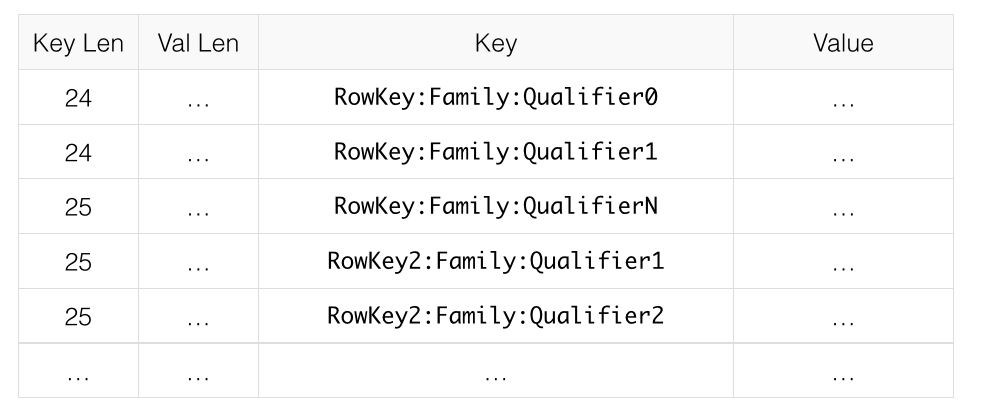
\includegraphics[width=0.7\textwidth]{figures/optimizations_no_encoding}
\caption{Column family stored with no encoding}
\label{figure:optimizations_no_encoding}
\end{figure}

Fast Diff works similar to Diff encoding, but uses a faster implementation. In Diff encoding, the most important feature is an extra column which holds the length of the prefix shared between the current key and the previous key. In addition, the timestamp is stored as the difference from the previous row's timestamp, rather than being stored in full. Figure \ref{figure:optimizations_diff_encoding} shows the same data with Figure \ref{figure:optimizations_no_encoding} stored with Diff encoding.

\begin{figure}[H]
\centering
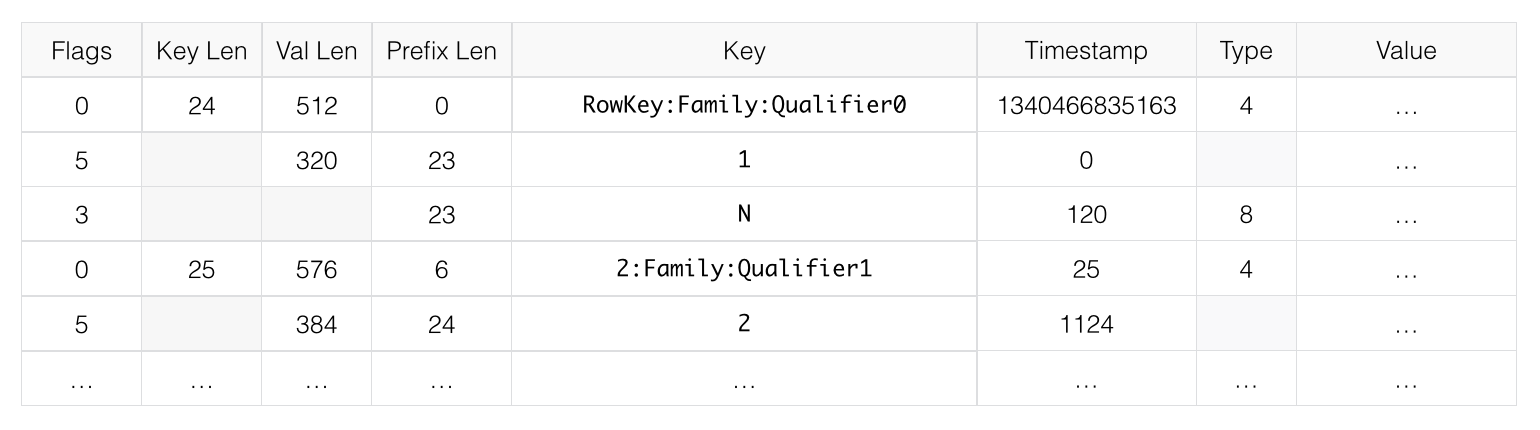
\includegraphics[width=\textwidth]{figures/optimizations_diff_encoding}
\caption{Column family stored with Diff encoding}
\label{figure:optimizations_diff_encoding}
\end{figure}

Both compression (with compressed BlockCache enabled) and data block encoding reduce the in-cache data size. This means that more rows can be cached at the same time, while data transfer time from the disk to the BlockCache for the same data is reduced. However every time the cached data is used in a query they must be decompressed or decoded or both. These performance hits increase query latency, while is our priority is to minimize it.

To achieve the best in-cache query latency we decide to use Snappy compression for our final Phoenix table, in conjunction with enabled compressed BlockCache and no data block encoding. The experiment on which we base this decision is presented on Subsection \ref{subsection:benchmarks_compression_encoding}.


\section{Disable BlockCache on the Reverse DNS Table}

The Reverse DNS dataset is stored in the \texttt{rdns} HBase table. This table has Snappy compression and no data block encoding to reduce on-disk size and avoid the decoding performance hit on read. The on-disk size of the compressed table is 12GB.

We investigate the read access pattern on the table by the IP to DNS Bolt. Since the IP addresses on the packets are random, the reads are performed on the table \texttt{rdns} are random too. Every read caches the HFile it hits, which does not provide any benefit since \texttt{rdns} does not fit into the BlockCaches of the RegionServers. Moreover, constantly caching different HFiles of \texttt{rdns} throws out of the cache HFiles of the output table \texttt{netdata}. Subsequent queries will have to cache these HFiles again, which increases the query latency.

To alleviate this problem we disable BlockCache on \texttt{rdns}, thus allowing the \texttt{netdata} table to fully take advantage of the cache.


\section{Salting}\label{section:optimizations_salting}

Rows in HBase are sorted lexicographically by row key. The row key for the HBase table where our Phoenix table is stored must be the timestamp associated with the packet, in order to optimize scans for queries over a specified time range. Since the timestamp is always increasing for live data, the row key is also monotonically increasing.

However, monotonically increasing row keys are a common source of hotspotting. When records with sequential keys are being written to HBase all writes hit one region which is served by one RegionServer. This uneven write load distribution limits the write throughput to the capacity of a single RegionServer instead of making use of multiple nodes in the HBase cluster. Moreover, hotspotting overwhelms the RegionServer responsible for hosting that region, causing performance degradation and potentially leading to region unavailability.

Salting the row key provides a way to mitigate the problem. Salting refers to adding a randomly-assigned prefix to the row key to cause it to sort differently than it otherwise would. The number of possible prefixes correspond to the number of regions you want to spread the data across. For example we can salt the row key by using this:

\begin{lstlisting}[language=C]
newKey = (++index % BUCKETS_NUMBER) + originalKey
\end{lstlisting}

In this listing, the \texttt{newKey} is produced by prefixing the \texttt{originalKey} a salt denoting the salt bucket. The salted records are be split into multiple buckets served by different RegionServers. The row keys of bucketed records are no longer in the original sequence, however records within in each bucket preserve their original sequence, as seen in Figure \ref{figure:optimizations_salting}.

\begin{figure}[H]
\centering
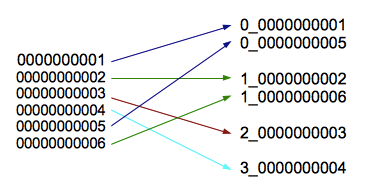
\includegraphics[width=0.6\textwidth]{figures/optimizations_salting}
\caption{HBase row key prefix salting}
\label{figure:optimizations_salting}
\end{figure}

Since data is placed in multiple buckets during writes, we have to read from all of those buckets when doing scans based on original start and stop keys and merge-sort the data. These scans can be run in parallel on the different RegionServers serving the salt buckets, which may lead to an increase in read performance.

Phoenix provides a way to transparently salt the row key with a salting byte for a particular table. To distribute the load evenly among all the nodes of the HBase cluster we set the number of salt buckets equal to the number of the RegionServers. The effect of salting on writes and reads is evaluated on Subsections \ref{subsection:benchmarks_storm_salting} and \ref{subsection:benchmarks_hbase_salting} respectively.


\cleardoublepage
